\chapter{Histórico}
\capepigrafe[0.5\textwidth]{I don't need a hard disk in my computer if I can get to the server faster... carrying around these non-connected computers is byzantine by comparison.}{Steve Jobs\cite{quotes}}

\section{Contexto}

\nocite{precloudcomputing}
A computação, em meados dos anos 90, consistia na evolução do computador pessoal e na consolidação da internet pelo mundo todo. A essência das aplicações construídas estava na distribuição de programas pela internet. Com o advento de aplicações web, torna-se necessário hospedar essas aplicações em servidores. Geralmente, era uma máquina física dedicada ao serviço, onde a aplicação ficaria hospedada, recebendo suas requisições.

\section{Problemas}

No contexto da época, esses servidores dedicados falhavam com certa frequência. Em casos de falha, o administrador do sistema precisava colocar uma nova máquina para atender a demanda, enquanto entendia a falha de \textit{software} ocorrida. Porém, toda a provisão de novos servidores para gerar redundância e tolerância a falhas aumentava a probabilidade de máquinas físicas falharem, gerando maiores problemas e dificuldades para manutenção.

\section{Primórdios}


Em 2006, a Amazon, percebendo a oportunidade de diversificar seu negócio atuando com provisionamento de infraestrutura, gerenciando máquinas ociosas de acordo com os horários possíveis e cuidando de toda a manutenção trabalhosa pelo lado do desenvolvedor, formulou e lançou a primeira versão do Amazon Elastic Compute Cloud (EC2), o primeiro produto voltado para a computação em nuvem, com o propósito de atender essa necessidade encontrada e vender infraestrutura para o usuário final.

\begin{figure}[h!]
  \centering
  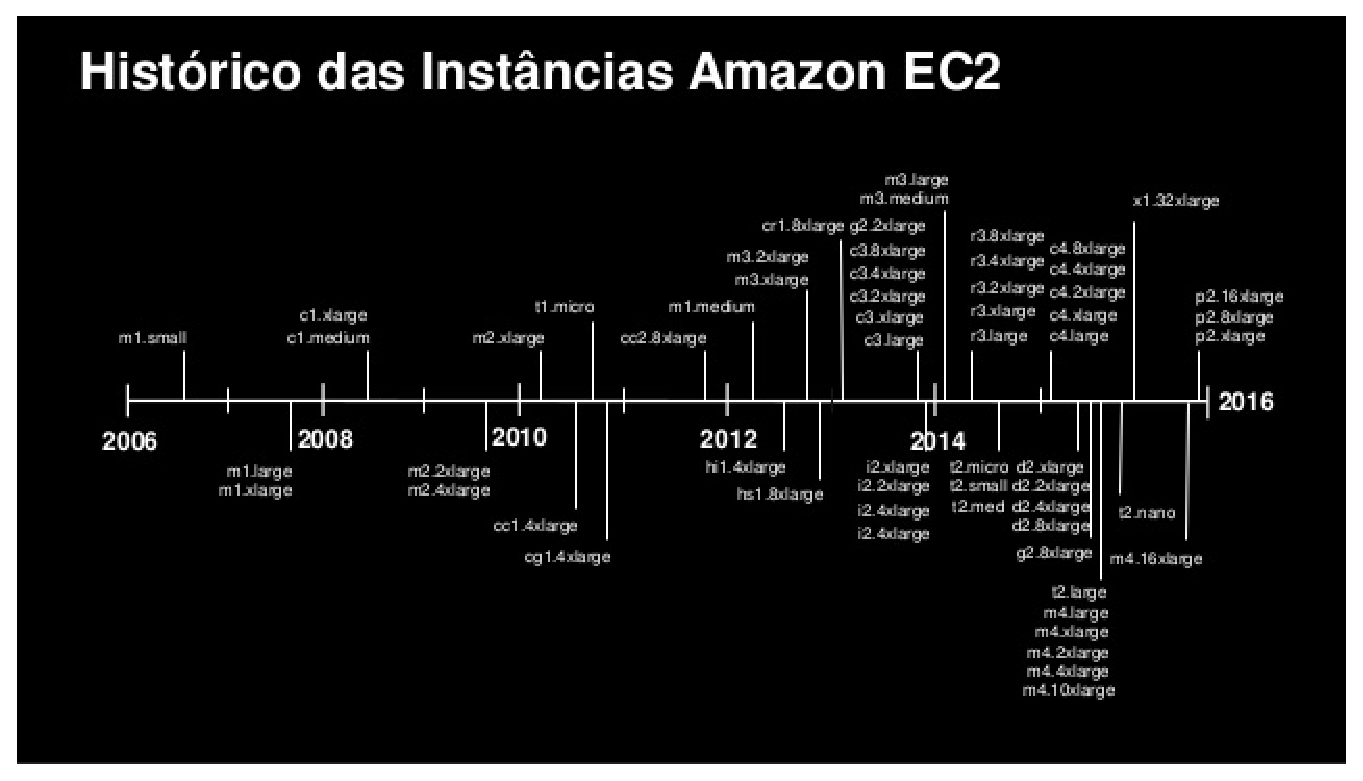
\includegraphics[scale=0.60]{imagens/ec2_history.eps}
  \caption{Histórico do Amazon EC2\cite{ec2history}}
\end{figure}

A postagem original no site da Amazon anunciava o serviço (em inglês)\cite{postamazonec2}:

\begin{citacaoLonga}
  Amazon Elastic Compute Cloud (Amazon EC2) is a web service that provides resizable compute capacity in the cloud. It is designed to make web-scale computing easier for developers. Just as Amazon Simple Storage Service (Amazon S3) enables storage in the cloud, Amazon EC2 enables “compute” in the cloud. Amazon EC2’s simple web service interface allows you to obtain and configure capacity with minimal friction. It provides you with complete control of your computing resources and lets you run on Amazon’s proven computing environment. Amazon EC2 reduces the time required to obtain and boot new server instances to minutes, allowing you to quickly scale capacity, both up and down, as your computing requirements change. Amazon EC2 changes the economics of computing by allowing you to pay only for capacity that you actually use.
\end{citacaoLonga}

\section{Impactos}

Essencialmente, a Amazon comercializou o conceito de infraestrutura como serviço (\textit{IaaS}). A revolução iniciada na época permitiu que muitas aplicações hospedadas em servidores físicos fossem migrados para a infraestrutura da Amazon. A cobrança realizada por hora de instância virtual carregada era bem inferior aos custos (tanto reais quanto de trabalho) de manter uma infraestrutura física equivalente, fora o fato de que a ociosidade foi drasticamente reduzida, pois o gerenciamento inteligente do EC2 permitia que uma mesma máquina atendesse dois serviços em horários distintos.

\begin{figure}[h!]
  \centering
  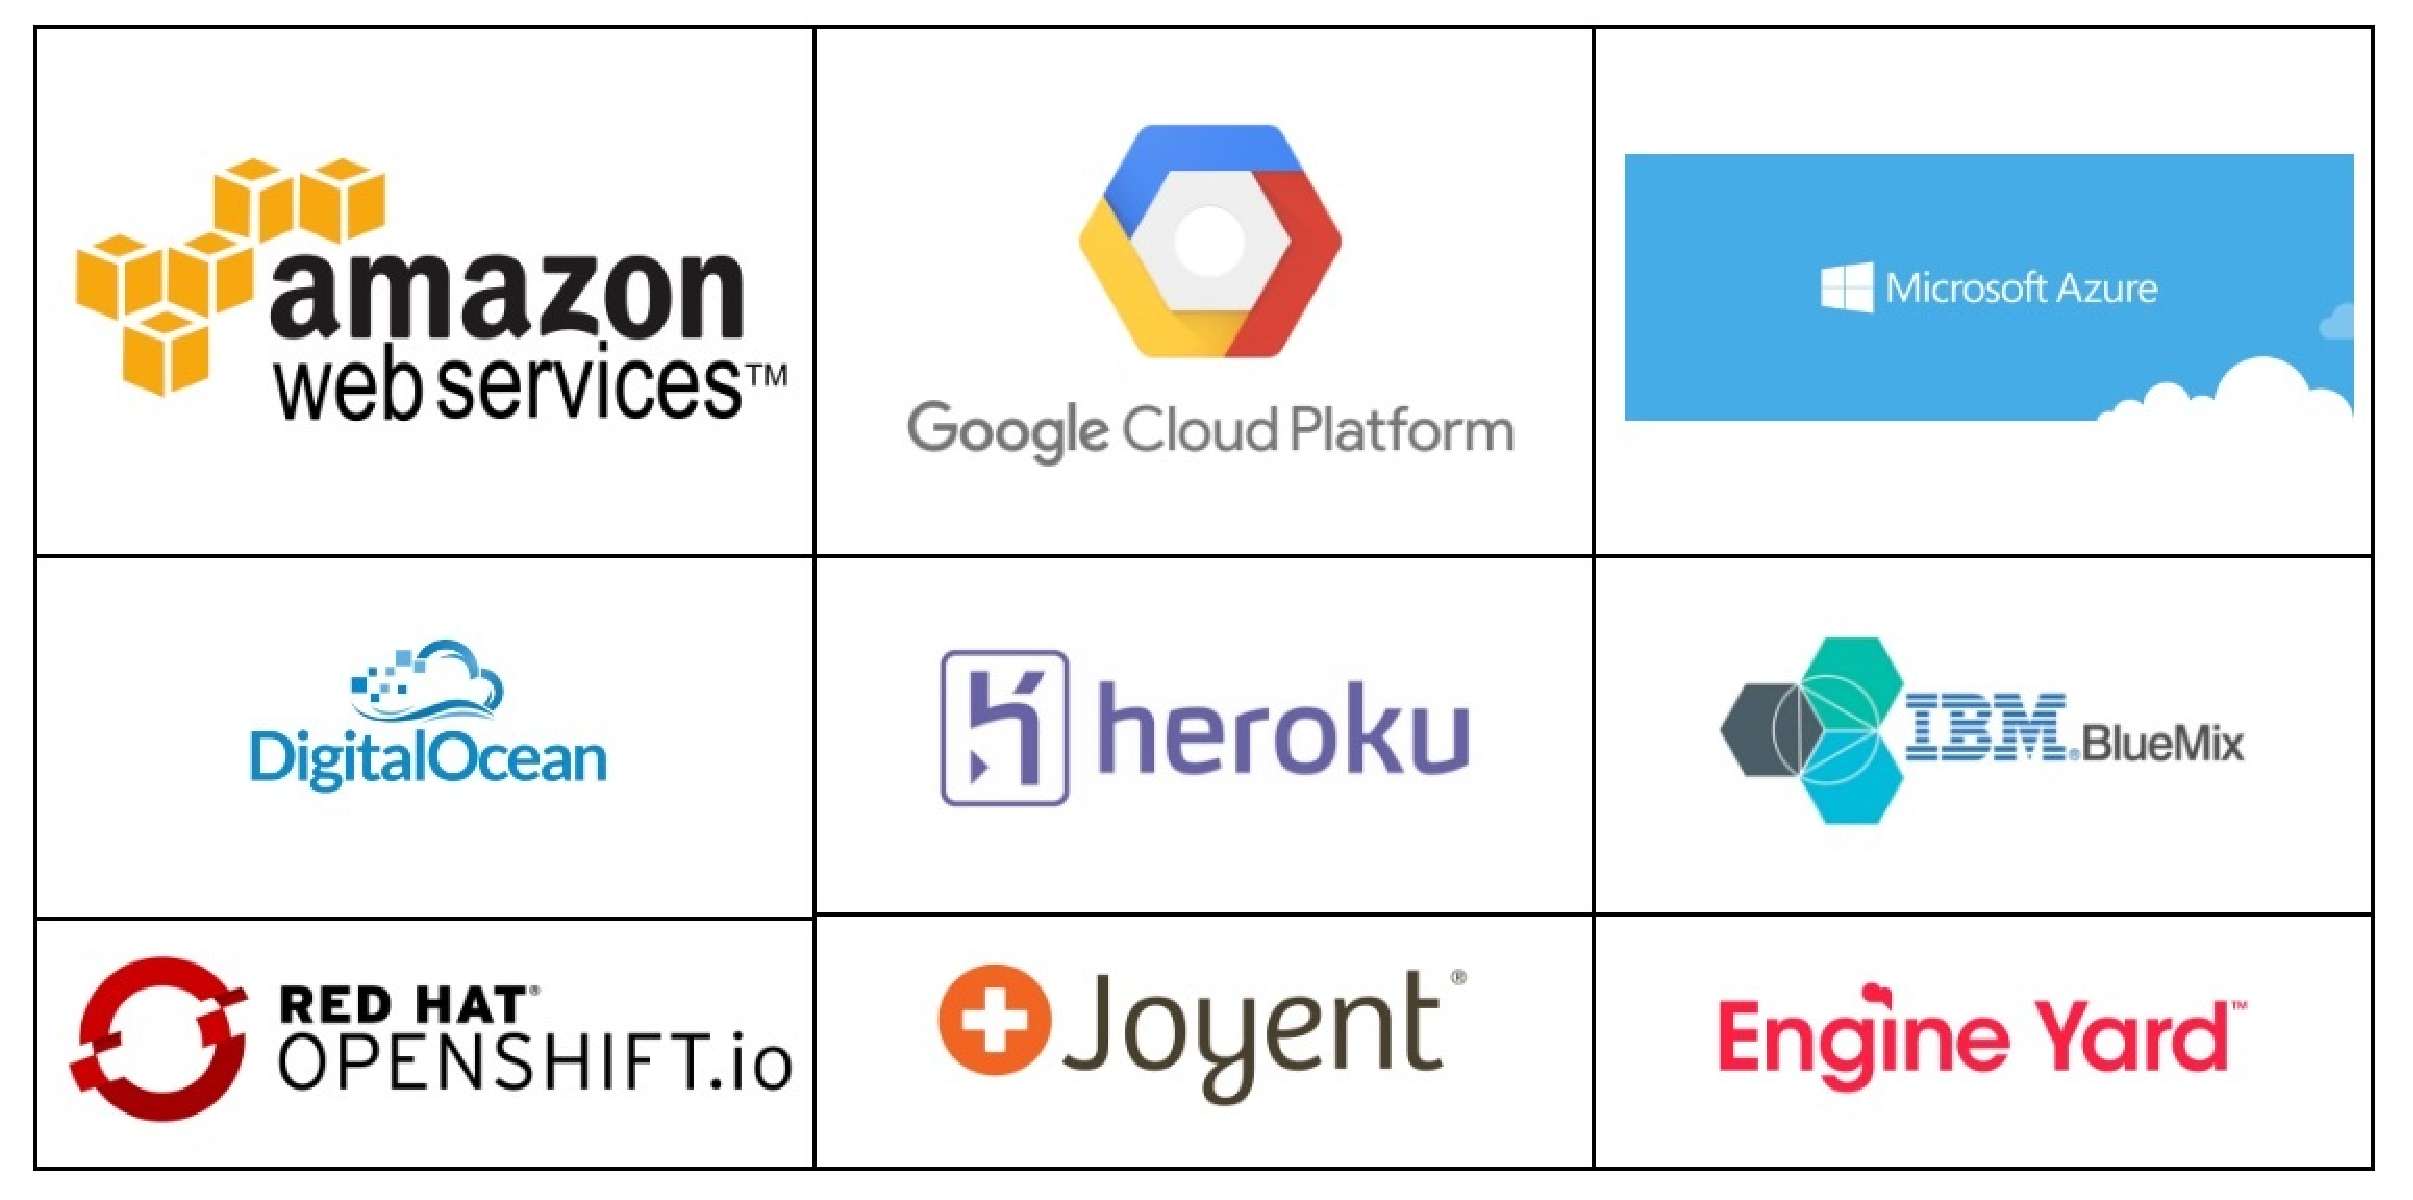
\includegraphics[scale=0.40]{imagens/clouds.eps}
  \caption{Algumas soluções de Computação em Nuvem\cite{clouds}}
\end{figure}

Com o trunfo do EC2, outras soluções ganharam força, merecendo destaque para: \textbf{Salesforce Heroku}, \textbf{Google Cloud} e \textbf{Microsoft Azure}, que serão exploradas adiante. Atualmente, a adoção, segundo o relatório anual de Computação em Nuvem da RightScale\cite{rightscale}, está em grande parte para a AWS:

\begin{figure}[h!]
  \centering
  \includegraphics[scale=0.20]{imagens/rightscale_cloud_adoption.eps}
  \caption{Adesão de serviços de computação em nuvem segundo a RightScale\cite{rightscale}}
\end{figure}
